\subsection{Geometry}
\label{subsection:algorithms_geometry}

Creating a 3D magnet geometry within a~CAD tool in which a~single cable is wound $n$ times is a~complicated task, because the model must take into account a relative position of one winding with respect to another. Therefore, every winding is considered to be a~separate domain in prepared ANSYS models with winding jumps, as shown in Fig. \ref{fig:winding_geom_scheme}. The green lines depict the electro-thermal coupling of windings according to their winding order. With such an approach, one can easily create multi-strand magnet geometries. Moreover, by specifying which windings are coupled together, with the same numerical domain, one can also analyse magnets with a different winding scheme.

\begin{figure}[H]
\centering
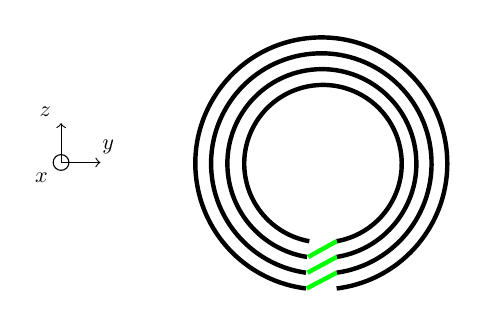
\begin{tikzpicture}[scale = 1.0]

    \draw [ultra thick] (0,0) arc (-80:260:1);
    \draw [ultra thick] (0,-0.2) arc (-81:261:1.2);
    \draw [ultra thick] (0,-0.4) arc (-82:262:1.4);
    \draw [ultra thick] (0,-0.6) arc (-83:263:1.6);
    
    \draw [ultra thick, green] (0,0) -- (-0.36,-0.2);
    \draw [ultra thick, green] (0,-0.2) -- (-0.37,-0.4);
    \draw [ultra thick, green] (0,-0.4) -- (-0.38,-0.6);
    
    \draw (-3.5,1) circle (0.1cm);
    \draw[black, ->] (-3.5,1) -- (-3.5,1.5);
    \draw[black, ->] (-3.5,1) -- (-3,1);
    
    \node[scale = 0.8] at (-3.75,0.8) {$x$};
    \node[scale = 0.8] at (-2.9,1.2) {$y$};
    \node[scale = 0.8] at (-3.7,1.65) {$z$};

\end{tikzpicture}
\caption{Domain representation with multiple windings.}
\label{fig:winding_geom_scheme}
\end{figure}

Every winding can have an external homogenised insulation layer represented as a~transverse one-dimensional element, as shown in Fig.~\ref{fig: insulation_coupling}. If multiple windings are created, the~end nodes of each insulation layer are thermally coupled with the neighbouring insulation elements. The~model assumes no diagonal heat propagation across the insulation layer, i.e. the~windings are not diagonally coupled. The insulation elements marked in blue are represented by the LINK33 element whereas the composite strand in yellow -- LINK68. LINK68 is a~uniaxial 1D element which can be used in a 3D space. It has the ability to conduct heat and electrical current along its nodes with an internal heat source corresponding to the Joule heating. LINK68 is used for steady-state and transient simulations. In standard ANSYS simulations, the Joule heating is implemented by introducing a power source over the entire strand domain as a function of resistivity (being a function of temperature). The usage of LINK68 in the quench velocity-based approach allows to omit applying the external power source since the solver computes the heat source by an~internal routine based on the material property state. Thus, the element requires electrical resistivity of the composite strand~\cite{ansys_element_manual}.

\begin{figure}[H]
    \centering
    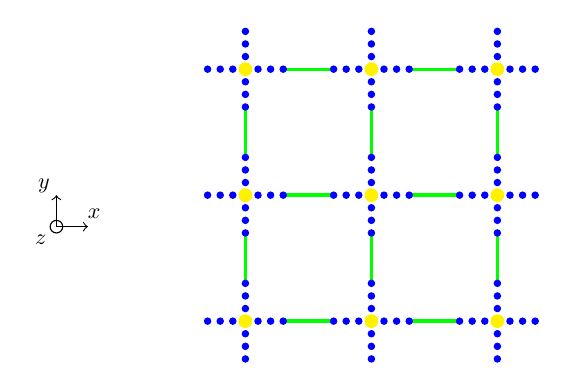
\begin{tikzpicture}[scale = 0.8]
        
        % coupling 
        \foreach \x in {0,2,4}
            \foreach \y in {3/5, 3/5+2}
                \draw[very thick, green] (\x, \y) -- (\x, -\y+2);
        \foreach \y in {0,2,4}
            \foreach \x in {3/5, 3/5+2}
                \draw[very thick, green] (\x, \y) -- (-\x+2, \y);
        
        % row number 1  
        \foreach \x in {-3,-2,...,3}
            \filldraw[blue] (\x/5, 0) circle (0.05);
        \foreach \y in {-3,-2,...,3}
            \filldraw[blue] (0, \y/5) circle (0.05);    
         \foreach \x in {-3,-2,...,3}
            \filldraw[blue] (\x/5+2, 0) circle (0.05);
        \foreach \y in {-3,-2,...,3}
            \filldraw[blue] (2, \y/5) circle (0.05);   
        \foreach \x in {-3,-2,...,3}
            \filldraw[blue] (\x/5+4, 0) circle (0.05);
        \foreach \y in {-3,-2,...,3}
            \filldraw[blue] (4, \y/5) circle (0.05);   
        
        % row number 2
        \foreach \x in {-3,-2,...,3}
            \filldraw[blue] (\x/5, 2) circle (0.05);
        \foreach \y in {-3,-2,...,3}
            \filldraw[blue] (0, \y/5+2) circle (0.05);    
         \foreach \x in {-3,-2,...,3}
            \filldraw[blue] (\x/5+2, 2) circle (0.05);
        \foreach \y in {-3,-2,...,3}
            \filldraw[blue] (2, \y/5+2) circle (0.05);   
        \foreach \x in {-3,-2,...,3}
            \filldraw[blue] (\x/5+4, 2) circle (0.05);
        \foreach \y in {-3,-2,...,3}
            \filldraw[blue] (4, \y/5+2) circle (0.05);   
        
        % row number 3
        \foreach \x in {-3,-2,...,3}
            \filldraw[blue] (\x/5, 4) circle (0.05);
        \foreach \y in {-3,-2,...,3}
            \filldraw[blue] (0, \y/5+4) circle (0.05);    
         \foreach \x in {-3,-2,...,3}
            \filldraw[blue] (\x/5+2, 4) circle (0.05);
        \foreach \y in {-3,-2,...,3}
            \filldraw[blue] (2, \y/5+4) circle (0.05);   
        \foreach \x in {-3,-2,...,3}
            \filldraw[blue] (\x/5+4, 4) circle (0.05);
        \foreach \y in {-3,-2,...,3}
            \filldraw[blue] (4, \y/5+4) circle (0.05);   
        \foreach \x in {0,2,4} 
            \foreach \y in {0,2,4} 
                \filldraw[yellow] (\x, \y) circle (0.1);
    \draw[scale=1] (-3.5+0.5,1+0.5) circle (0.1cm);
    \draw[black, ->, scale=1] (-3.5+0.5,1+0.5) -- (-3.5+0.5,1.5+0.5);
    \draw[black, ->, scale=1] (-3.5+0.5,1+0.5) -- (-3+0.5,1+0.5);
    \node[scale = 0.8] at (-3.75+0.5,0.8+0.5) {$z$};
    \node[scale = 0.8] at (-2.9+0.5,1.2+0.5) {$x$};
    \node[scale = 0.8] at (-3.7+0.5,1.65+0.5) {$y$};
        
    \end{tikzpicture}
    \caption{Cross-section of a 1D+1D+1D geometry with coupled insulation nodes marked in green.}
    \label{fig: insulation_coupling}
\end{figure}

\subsection{Mesh Generation}

The~mesh generation scheme for the~magnet geometry is illustrated in Fig.~\ref{fig: mesh_generation_in_multidimensional_case}. The~mesh should be distributed over so called "nodal planes", which are always perpendicular to the~normal vector $\vec{n}$ of a directional spline. The directional spline is a curve that represents a final shape of the coil. One nodal plane with nine windings is presented in Fig.~\ref{fig: insulation_coupling}. In order to generate mesh, a~longitudinal number of divisions has to be specified. When the insulation is considered, the number of divisions across the insulation must be defined as well. Each insulation element is characterised by the same volume. 

\begin{figure}[H]
    \centering
    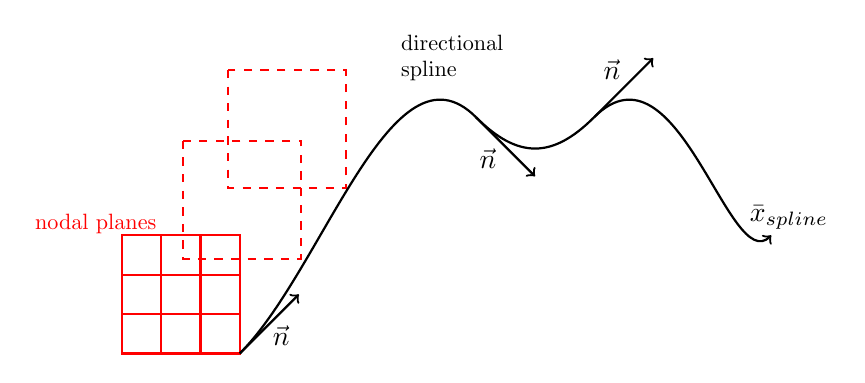
\begin{tikzpicture}[scale = 1.5]
        
        \draw[thick, red] (-1,1) rectangle (0,0);
        \draw[thick, red] (-1,1/3) -- (0,1/3);
        \draw[thick, red] (-1,2/3) -- (0,2/3);
        \draw[thick, red] (-1/3,0) -- (-1/3,1);
        \draw[thick, red] (-2/3,0) -- (-2/3,1);
        
        \draw[thick, red, dashed, xshift=0.52cm, yshift=0.8cm] (-1,1) rectangle (0,0);
        \draw[thick, red, dashed, xshift=0.9cm, yshift=1.4cm] (-1,1) rectangle (0,0);
        
        \draw[thick, black] (0,0) .. controls +(45:1cm) and +(135:1cm) .. (2,2);
        \draw[thick, black] (2,2) .. controls +(135:-0.5cm) and +(45:-0.5cm) .. (3,2);
        \draw[thick, black, ->] (3,2) .. controls +(45:1cm) and +(45:-0.5cm) .. (4.5,1);
        
        \draw[thick, black, ->] (0,0) -- (0.5,0.5);
        \draw[thick, black, ->] (2,2) -- (2.5,1.5);
        \draw[thick, black, ->] (3,2) -- (3.5,2.5);

        \node[red, scale=0.8, text width=2cm] at (-1.2,1.1) {nodal planes};
        \node[black, scale=0.8, text width=2cm] at (1.9,2.5) {directional spline};
        \node[black] at (0.35,0.15) {$\vec{n}$};
        \node[black] at (2.1,1.65) {$\vec{n}$};
        \node[black] at (3.15,2.4) {$\vec{n}$};
        
        \node[scale = 1.0] at (4.65,1.15) {$\bar x_\text{spline}$};

    \end{tikzpicture}
    \caption{Multidimensional mesh generation.}
    \label{fig: mesh_generation_in_multidimensional_case}
\end{figure}
